\chapter{Tìm kiếm toàn diện}

\key{Tìm kiếm toàn diện}
là một phương pháp tổng quát có thể được sử dụng
để giải quyết hầu hết mọi bài toán thuật toán.
Ý tưởng là tạo ra tất cả các giải pháp
có thể cho bài toán bằng cách duyệt trâu,
và sau đó chọn giải pháp tốt nhất hoặc đếm
số lượng giải pháp, tùy thuộc vào bài toán.

Tìm kiếm toàn diện là một kỹ thuật tốt
nếu có đủ thời gian để duyệt qua tất cả các giải pháp,
bởi vì việc tìm kiếm thường dễ cài đặt
và nó luôn cho ra câu trả lời đúng.
Nếu tìm kiếm toàn diện quá chậm,
các kỹ thuật khác, chẳng hạn như thuật toán tham lam hoặc
quy hoạch động, có thể cần thiết.

\section{Tạo tập con}

\index{tập con}

Đầu tiên, chúng ta xem xét bài toán tạo
tất cả các tập con của một tập hợp gồm $n$ phần tử.
Ví dụ, các tập con của $\{0,1,2\}$ là
$\emptyset$, $\{0\}$, $\{1\}$, $\{2\}$, $\{0,1\}$,
$\{0,2\}$, $\{1,2\}$ và $\{0,1,2\}$.
Có hai phương pháp phổ biến để tạo tập con:
chúng ta có thể thực hiện tìm kiếm đệ quy
hoặc khai thác biểu diễn bit của các số nguyên.

\subsubsection{Phương pháp 1}

Một cách thanh lịch để duyệt qua tất cả các tập con
của một tập hợp là sử dụng đệ quy.
Hàm \texttt{search} sau đây
tạo ra các tập con của tập hợp
$\{0,1,\ldots,n-1\}$.
Hàm duy trì một vector \texttt{subset}
sẽ chứa các phần tử của mỗi tập con.
Việc tìm kiếm bắt đầu khi hàm được gọi
với tham số 0.

\begin{lstlisting}
void search(int k) {
    if (k == n) {
        // xu ly tap con
    } else {
        search(k+1);
        subset.push_back(k);
        search(k+1);
        subset.pop_back();
    }
}
\end{lstlisting}

Khi hàm \texttt{search}
được gọi với tham số $k$,
nó quyết định có bao gồm
phần tử $k$ trong tập con hay không,
và trong cả hai trường hợp,
sau đó gọi chính nó với tham số $k+1$.
Tuy nhiên, nếu $k=n$, hàm nhận thấy rằng
tất cả các phần tử đã được xử lý
và một tập con đã được tạo ra.

Cây sau đây minh họa các lệnh gọi hàm khi $n=3$.
Chúng ta luôn có thể chọn nhánh bên trái
($k$ không được bao gồm trong tập con) hoặc nhánh bên phải
($k$ được bao gồm trong tập con).

\begin{center}
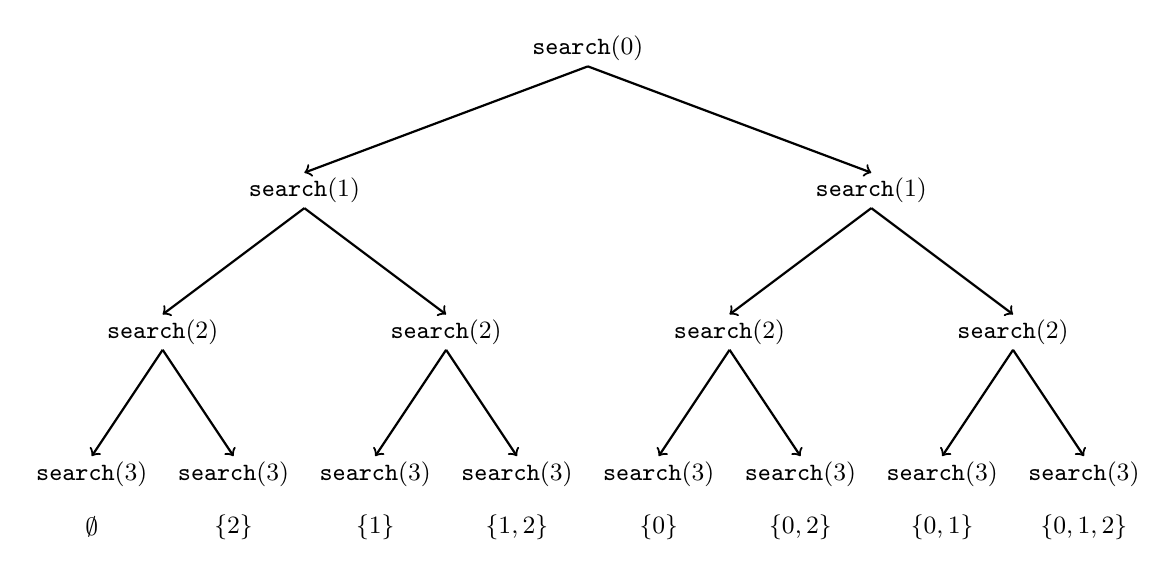
\begin{tikzpicture}[scale=.45]
  \begin{scope}
    \small
    \node at (0,0) {$\texttt{search}(0)$};

    \node at (-8,-4) {$\texttt{search}(1)$};
    \node at (8,-4) {$\texttt{search}(1)$};

    \path[draw,thick,->] (0,0-0.5) -- (-8,-4+0.5);
    \path[draw,thick,->] (0,0-0.5) -- (8,-4+0.5);

    \node at (-12,-8) {$\texttt{search}(2)$};
    \node at (-4,-8) {$\texttt{search}(2)$};
    \node at (4,-8) {$\texttt{search}(2)$};
    \node at (12,-8) {$\texttt{search}(2)$};

    \path[draw,thick,->] (-8,-4-0.5) -- (-12,-8+0.5);
    \path[draw,thick,->] (-8,-4-0.5) -- (-4,-8+0.5);
    \path[draw,thick,->] (8,-4-0.5) -- (4,-8+0.5);
    \path[draw,thick,->] (8,-4-0.5) -- (12,-8+0.5);

    \node at (-14,-12) {$\texttt{search}(3)$};
    \node at (-10,-12) {$\texttt{search}(3)$};
    \node at (-6,-12) {$\texttt{search}(3)$};
    \node at (-2,-12) {$\texttt{search}(3)$};
    \node at (2,-12) {$\texttt{search}(3)$};
    \node at (6,-12) {$\texttt{search}(3)$};
    \node at (10,-12) {$\texttt{search}(3)$};
    \node at (14,-12) {$\texttt{search}(3)$};

    \node at (-14,-13.5) {$\emptyset$};
    \node at (-10,-13.5) {$\{2\}$};
    \node at (-6,-13.5) {$\{1\}$};
    \node at (-2,-13.5) {$\{1,2\}$};
    \node at (2,-13.5) {$\{0\}$};
    \node at (6,-13.5) {$\{0,2\}$};
    \node at (10,-13.5) {$\{0,1\}$};
    \node at (14,-13.5) {$\{0,1,2\}$};


    \path[draw,thick,->] (-12,-8-0.5) -- (-14,-12+0.5);
    \path[draw,thick,->] (-12,-8-0.5) -- (-10,-12+0.5);
    \path[draw,thick,->] (-4,-8-0.5) -- (-6,-12+0.5);
    \path[draw,thick,->] (-4,-8-0.5) -- (-2,-12+0.5);
    \path[draw,thick,->] (4,-8-0.5) -- (2,-12+0.5);
    \path[draw,thick,->] (4,-8-0.5) -- (6,-12+0.5);
    \path[draw,thick,->] (12,-8-0.5) -- (10,-12+0.5);
    \path[draw,thick,->] (12,-8-0.5) -- (14,-12+0.5);
\end{scope}
\end{tikzpicture}
\end{center}

\subsubsection{Phương pháp 2}

Một cách khác để tạo tập con là dựa trên
biểu diễn bit của các số nguyên.
Mỗi tập con của một tập hợp gồm $n$ phần tử
có thể được biểu diễn dưới dạng một chuỗi $n$ bit,
tương ứng với một số nguyên từ $0 \ldots 2^n-1$.
Các bit một trong chuỗi bit cho biết
phần tử nào được bao gồm trong tập con.

Quy ước thông thường là
bit cuối cùng tương ứng với phần tử 0,
bit thứ hai cuối cùng tương ứng với phần tử 1,
vân vân.
Ví dụ, biểu diễn bit của 25 là 11001,
tương ứng với tập con $\{0,3,4\}$.

Đoạn mã sau duyệt qua các tập con
của một tập hợp gồm $n$ phần tử

\begin{lstlisting}
for (int b = 0; b < (1<<n); b++) {
    // xu ly tap con
}
\end{lstlisting}

Đoạn mã sau cho thấy cách chúng ta có thể tìm
các phần tử của một tập con tương ứng với một chuỗi bit.
Khi xử lý mỗi tập con,
đoạn mã xây dựng một vector chứa các
phần tử trong tập con.

\begin{lstlisting}
for (int b = 0; b < (1<<n); b++) {
    vector<int> subset;
    for (int i = 0; i < n; i++) {
        if (b&(1<<i)) subset.push_back(i);
    }
}
\end{lstlisting}

\section{Tạo hoán vị}

\index{hoán vị}

Tiếp theo, chúng ta xem xét bài toán tạo
tất cả các hoán vị của một tập hợp gồm $n$ phần tử.
Ví dụ, các hoán vị của $\{0,1,2\}$ là
$(0,1,2)$, $(0,2,1)$, $(1,0,2)$, $(1,2,0)$,
$(2,0,1)$ và $(2,1,0)$.
Một lần nữa, có hai cách tiếp cận:
chúng ta có thể sử dụng đệ quy hoặc duyệt qua các
hoán vị một cách lặp đi lặp lại.

\subsubsection{Phương pháp 1}

Giống như tập con, hoán vị có thể được tạo ra
bằng cách sử dụng đệ quy.
Hàm \texttt{search} sau đây duyệt qua
các hoán vị của tập hợp $\{0,1,\ldots,n-1\}$.
Hàm xây dựng một vector \texttt{permutation}
chứa hoán vị,
và việc tìm kiếm bắt đầu khi hàm được
gọi mà không có tham số.

\begin{lstlisting}
void search() {
    if (permutation.size() == n) {
        // xu ly hoan vi
    } else {
        for (int i = 0; i < n; i++) {
            if (chosen[i]) continue;
            chosen[i] = true;
            permutation.push_back(i);
            search();
            chosen[i] = false;
            permutation.pop_back();
        }
    }
}
\end{lstlisting}

Mỗi lệnh gọi hàm thêm một phần tử mới vào
\texttt{permutation}.
Mảng \texttt{chosen} cho biết
phần tử nào đã được bao gồm trong hoán vị.
Nếu kích thước của \texttt{permutation} bằng kích thước của tập hợp,
một hoán vị đã được tạo ra.

\subsubsection{Phương pháp 2}

\index{next\_permutation@\texttt{next\_permutation}}

Một phương pháp khác để tạo hoán vị
là bắt đầu với hoán vị
$\{0,1,\ldots,n-1\}$ và lặp đi lặp lại
sử dụng một hàm xây dựng hoán vị tiếp theo
theo thứ tự tăng dần.
Thư viện chuẩn C++ chứa hàm
\texttt{next\_permutation} có thể được sử dụng cho việc này:

\begin{lstlisting}
vector<int> permutation;
for (int i = 0; i < n; i++) {
    permutation.push_back(i);
}
do {
    // xu ly hoan vi
} while (next_permutation(permutation.begin(),permutation.end()));
\end{lstlisting}

\section{Quay lui}

\index{quay lui}

Một thuật toán \key{quay lui}
bắt đầu với một giải pháp rỗng
và mở rộng giải pháp từng bước.
Việc tìm kiếm đệ quy
duyệt qua tất cả các cách khác nhau để
xây dựng một giải pháp.

\index{bài toán quân hậu}

Ví dụ, hãy xem xét bài toán
tính số cách
$n$ quân hậu có thể được đặt trên
bàn cờ $n \times n$ sao cho
không có hai quân hậu nào tấn công nhau.
Ví dụ, khi $n=4$,
có hai giải pháp khả thi:

\begin{center}
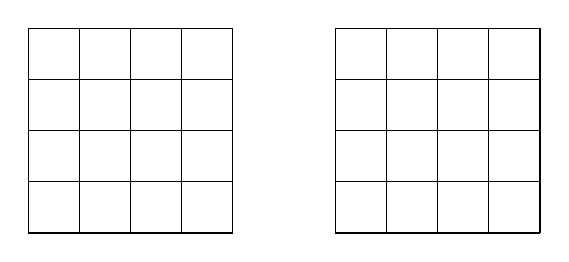
\begin{tikzpicture}[scale=.65]
  \begin{scope}
    \draw (0, 0) grid (4, 4);
    \node at (1.5,3.5) {\symqueen};
    \node at (3.5,2.5) {\symqueen};
    \node at (0.5,1.5) {\symqueen};
    \node at (2.5,0.5) {\symqueen};

    \draw (6, 0) grid (10, 4);
    \node at (6+2.5,3.5) {\symqueen};
    \node at (6+0.5,2.5) {\symqueen};
    \node at (6+3.5,1.5) {\symqueen};
    \node at (6+1.5,0.5) {\symqueen};

  \end{scope}
\end{tikzpicture}
\end{center}

Bài toán có thể được giải quyết bằng cách sử dụng quay lui
bằng cách đặt các quân hậu lên bàn cờ theo từng hàng.
Chính xác hơn, chính xác một quân hậu sẽ
được đặt trên mỗi hàng sao cho không có quân hậu nào tấn công
bất kỳ quân hậu nào được đặt trước đó.
Một giải pháp đã được tìm thấy khi tất cả
$n$ quân hậu đã được đặt trên bàn cờ.

Ví dụ, khi $n=4$,
một số giải pháp một phần được tạo ra bởi
thuật toán quay lui như sau:

\begin{center}
\begin{tikzpicture}[scale=.55]
  \begin{scope}
    \draw (0, 0) grid (4, 4);

    \draw (-9, -6) grid (-5, -2);
    \draw (-3, -6) grid (1, -2);
    \draw (3, -6) grid (7, -2);
    \draw (9, -6) grid (13, -2);

    \node at (-9+0.5,-3+0.5) {\symqueen};
    \node at (-3+1+0.5,-3+0.5) {\symqueen};
    \node at (3+2+0.5,-3+0.5) {\symqueen};
    \node at (9+3+0.5,-3+0.5) {\symqueen};

    \draw (2,0) -- (-7,-2);
    \draw (2,0) -- (-1,-2);
    \draw (2,0) -- (5,-2);
    \draw (2,0) -- (11,-2);

    \draw (-11, -12) grid (-7, -8);
    \draw (-6, -12) grid (-2, -8);
    \draw (-1, -12) grid (3, -8);
    \draw (4, -12) grid (8, -8);
    \draw[white] (11, -12) grid (15, -8);
    \node at (-11+1+0.5,-9+0.5) {\symqueen};
    \node at (-6+1+0.5,-9+0.5) {\symqueen};
    \node at (-1+1+0.5,-9+0.5) {\symqueen};
    \node at (4+1+0.5,-9+0.5) {\symqueen};
    \node at (-11+0+0.5,-10+0.5) {\symqueen};
    \node at (-6+1+0.5,-10+0.5) {\symqueen};
    \node at (-1+2+0.5,-10+0.5) {\symqueen};
    \node at (4+3+0.5,-10+0.5) {\symqueen};

    \draw (-1,-6) -- (-9,-8);
    \draw (-1,-6) -- (-4,-8);
    \draw (-1,-6) -- (1,-8);
    \draw (-1,-6) -- (6,-8);

    \node at (-9,-13) {bất hợp lệ};
    \node at (-4,-13) {bất hợp lệ};
    \node at (1,-13) {bất hợp lệ};
    \node at (6,-13) {hợp lệ};

  \end{scope}
\end{tikzpicture}
\end{center}

Ở cấp dưới cùng, ba cấu hình đầu tiên
là bất hợp lệ, vì các quân hậu tấn công nhau.
Tuy nhiên, cấu hình thứ tư là hợp lệ
và nó có thể được mở rộng thành một giải pháp hoàn chỉnh bằng cách
đặt thêm hai quân hậu nữa lên bàn cờ.
Chỉ có một cách để đặt hai quân hậu còn lại.

\begin{samepage}
Thuật toán có thể được cài đặt như sau:
\begin{lstlisting}
void search(int y) {
    if (y == n) {
        count++;
        return;
    }
    for (int x = 0; x < n; x++) {
        if (column[x] || diag1[x+y] || diag2[x-y+n-1]) continue;
        column[x] = diag1[x+y] = diag2[x-y+n-1] = 1;
        search(y+1);
        column[x] = diag1[x+y] = diag2[x-y+n-1] = 0;
    }
}
\end{lstlisting}
\end{samepage}
Việc tìm kiếm bắt đầu bằng cách gọi \texttt{search(0)}.
Kích thước của bàn cờ là $n \times n$,
và đoạn mã tính số lượng giải pháp
vào \texttt{count}.

Đoạn mã giả định rằng các hàng và cột
của bàn cờ được đánh số từ 0 đến $n-1$.
Khi hàm \texttt{search} được
gọi với tham số $y$,
nó đặt một quân hậu trên hàng $y$
và sau đó gọi chính nó với tham số $y+1$.
Sau đó, nếu $y=n$, một giải pháp đã được tìm thấy
và biến \texttt{count} được tăng lên một.

Mảng \texttt{column} theo dõi các cột
chứa một quân hậu,
và các mảng \texttt{diag1} và \texttt{diag2}
theo dõi các đường chéo.
Không được phép thêm một quân hậu khác vào một
cột hoặc đường chéo đã chứa một quân hậu.
Ví dụ, các cột và đường chéo của
bàn cờ $4 \times 4$ được đánh số như sau:

\begin{center}
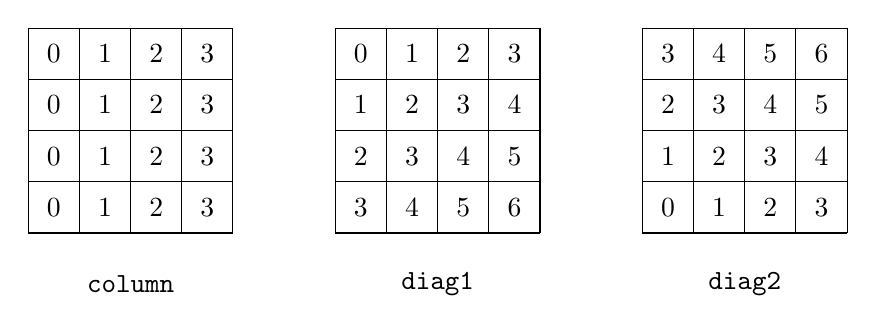
\begin{tikzpicture}[scale=.65]
  \begin{scope}
    \draw (0-6, 0) grid (4-6, 4);
    \node at (-6+0.5,3.5) {$0$};
    \node at (-6+1.5,3.5) {$1$};
    \node at (-6+2.5,3.5) {$2$};
    \node at (-6+3.5,3.5) {$3$};
    \node at (-6+0.5,2.5) {$0$};
    \node at (-6+1.5,2.5) {$1$};
    \node at (-6+2.5,2.5) {$2$};
    \node at (-6+3.5,2.5) {$3$};
    \node at (-6+0.5,1.5) {$0$};
    \node at (-6+1.5,1.5) {$1$};
    \node at (-6+2.5,1.5) {$2$};
    \node at (-6+3.5,1.5) {$3$};
    \node at (-6+0.5,0.5) {$0$};
    \node at (-6+1.5,0.5) {$1$};
    \node at (-6+2.5,0.5) {$2$};
    \node at (-6+3.5,0.5) {$3$};

    \draw (0, 0) grid (4, 4);
    \node at (0.5,3.5) {$0$};
    \node at (1.5,3.5) {$1$};
    \node at (2.5,3.5) {$2$};
    \node at (3.5,3.5) {$3$};
    \node at (0.5,2.5) {$1$};
    \node at (1.5,2.5) {$2$};
    \node at (2.5,2.5) {$3$};
    \node at (3.5,2.5) {$4$};
    \node at (0.5,1.5) {$2$};
    \node at (1.5,1.5) {$3$};
    \node at (2.5,1.5) {$4$};
    \node at (3.5,1.5) {$5$};
    \node at (0.5,0.5) {$3$};
    \node at (1.5,0.5) {$4$};
    \node at (2.5,0.5) {$5$};
    \node at (3.5,0.5) {$6$};

    \draw (6, 0) grid (10, 4);
    \node at (6.5,3.5) {$3$};
    \node at (7.5,3.5) {$4$};
    \node at (8.5,3.5) {$5$};
    \node at (9.5,3.5) {$6$};
    \node at (6.5,2.5) {$2$};
    \node at (7.5,2.5) {$3$};
    \node at (8.5,2.5) {$4$};
    \node at (9.5,2.5) {$5$};
    \node at (6.5,1.5) {$1$};
    \node at (7.5,1.5) {$2$};
    \node at (8.5,1.5) {$3$};
    \node at (9.5,1.5) {$4$};
    \node at (6.5,0.5) {$0$};
    \node at (7.5,0.5) {$1$};
    \node at (8.5,0.5) {$2$};
    \node at (9.5,0.5) {$3$};

    \node at (-4,-1) {\texttt{column}};
    \node at (2,-1) {\texttt{diag1}};
    \node at (8,-1) {\texttt{diag2}};

  \end{scope}
\end{tikzpicture}
\end{center}

Gọi $q(n)$ là số cách
đặt $n$ quân hậu trên bàn cờ $n \times n$.
Thuật toán quay lui ở trên
cho chúng ta biết rằng, ví dụ, $q(8)=92$.
Khi $n$ tăng, việc tìm kiếm nhanh chóng trở nên chậm,
vì số lượng giải pháp tăng
theo cấp số nhân.
Ví dụ, tính $q(16)=14772512$
sử dụng thuật toán trên đã mất khoảng một phút
trên một máy tính hiện đại\footnote{Không có cách nào được biết để tính toán hiệu quả
các giá trị lớn hơn của $q(n)$. Kỷ lục hiện tại là
$q(27)=234907967154122528$, được tính vào năm 2016 \cite{q27}.}.

\section{Cắt tỉa tìm kiếm}

Chúng ta thường có thể tối ưu hóa quay lui
bằng cách cắt tỉa cây tìm kiếm.
Ý tưởng là thêm "trí thông minh" vào thuật toán
để nó sẽ nhận ra càng sớm càng tốt
nếu một giải pháp một phần không thể được mở rộng
thành một giải pháp hoàn chỉnh.
Những tối ưu hóa như vậy có thể có một tác động to lớn
đến hiệu quả của việc tìm kiếm.

Hãy xem xét bài toán
tính số lượng đường đi
trong một lưới $n \times n$ từ góc trên bên trái
đến góc dưới bên phải sao cho
đường đi thăm mỗi ô vuông đúng một lần.
Ví dụ, trong một lưới $7 \times 7$,
có 111712 đường đi như vậy.
Một trong những đường đi như sau:

\begin{center}
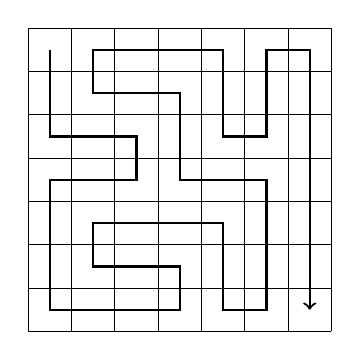
\begin{tikzpicture}[scale=.55]
  \begin{scope}
    \draw (0, 0) grid (7, 7);
    \draw[thick,->] (0.5,6.5) -- (0.5,4.5) -- (2.5,4.5) --
          (2.5,3.5) -- (0.5,3.5) -- (0.5,0.5) --
          (3.5,0.5) -- (3.5,1.5) -- (1.5,1.5) --
          (1.5,2.5) -- (4.5,2.5) -- (4.5,0.5) --
          (5.5,0.5) -- (5.5,3.5) -- (3.5,3.5) --
          (3.5,5.5) -- (1.5,5.5) -- (1.5,6.5) --
          (4.5,6.5) -- (4.5,4.5) -- (5.5,4.5) --
          (5.5,6.5) -- (6.5,6.5) -- (6.5,0.5);
  \end{scope}
\end{tikzpicture}
\end{center}

Chúng ta tập trung vào trường hợp $7 \times 7$,
vì mức độ khó của nó phù hợp với nhu cầu của chúng ta.
Chúng ta bắt đầu với một thuật toán quay lui đơn giản,
và sau đó tối ưu hóa nó từng bước bằng cách sử dụng các quan sát
về cách tìm kiếm có thể được cắt tỉa.
Sau mỗi lần tối ưu hóa, chúng ta đo thời gian chạy
của thuật toán và số lượng lệnh gọi đệ quy,
để chúng ta thấy rõ tác dụng của mỗi
lần tối ưu hóa đối với hiệu quả của việc tìm kiếm.

\subsubsection{Thuật toán cơ bản}

Phiên bản đầu tiên của thuật toán không chứa
bất kỳ tối ưu hóa nào. Chúng ta chỉ đơn giản sử dụng quay lui để tạo ra
tất cả các đường đi có thể từ góc trên bên trái đến
góc dưới bên phải và đếm số lượng các đường đi đó.

\begin{itemize}
\item
thời gian chạy: 483 giây
\item
số lượng lệnh gọi đệ quy: 76 tỷ
\end{itemize}

\subsubsection{Tối ưu hóa 1}

Trong bất kỳ giải pháp nào, chúng ta trước tiên di chuyển một bước
xuống hoặc sang phải.
Luôn có hai đường đi đối xứng
qua đường chéo của lưới
sau bước đầu tiên.
Ví dụ, các đường đi sau đây là đối xứng:

\begin{center}
\begin{tabular}{ccc}
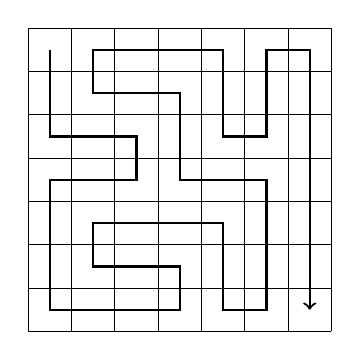
\begin{tikzpicture}[scale=.55]
  \begin{scope}
    \draw (0, 0) grid (7, 7);
    \draw[thick,->] (0.5,6.5) -- (0.5,4.5) -- (2.5,4.5) --
          (2.5,3.5) -- (0.5,3.5) -- (0.5,0.5) --
          (3.5,0.5) -- (3.5,1.5) -- (1.5,1.5) --
          (1.5,2.5) -- (4.5,2.5) -- (4.5,0.5) --
          (5.5,0.5) -- (5.5,3.5) -- (3.5,3.5) --
          (3.5,5.5) -- (1.5,5.5) -- (1.5,6.5) --
          (4.5,6.5) -- (4.5,4.5) -- (5.5,4.5) --
          (5.5,6.5) -- (6.5,6.5) -- (6.5,0.5);
  \end{scope}
\end{tikzpicture}
& \hspace{20px}
& 
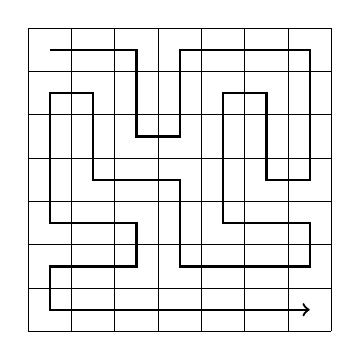
\begin{tikzpicture}[scale=.55]
  \begin{scope}[yscale=1,xscale=-1,rotate=-90]
    \draw (0, 0) grid (7, 7);
    \draw[thick,->] (0.5,6.5) -- (0.5,4.5) -- (2.5,4.5) --
          (2.5,3.5) -- (0.5,3.5) -- (0.5,0.5) --
          (3.5,0.5) -- (3.5,1.5) -- (1.5,1.5) --
          (1.5,2.5) -- (4.5,2.5) -- (4.5,0.5) --
          (5.5,0.5) -- (5.5,3.5) -- (3.5,3.5) --
          (3.5,5.5) -- (1.5,5.5) -- (1.5,6.5) --
          (4.5,6.5) -- (4.5,4.5) -- (5.5,4.5) --
          (5.5,6.5) -- (6.5,6.5) -- (6.5,0.5);
  \end{scope}
\end{tikzpicture}
\end{tabular}
\end{center}

Do đó, chúng ta có thể quyết định rằng chúng ta luôn luôn di chuyển trước
một bước xuống (hoặc sang phải),
và cuối cùng nhân số lượng giải pháp với hai.

\begin{itemize}
\item
thời gian chạy: 244 giây
\item
số lượng lệnh gọi đệ quy: 38 tỷ
\end{itemize}

\subsubsection{Tối ưu hóa 2}

Nếu đường đi đến ô vuông dưới cùng bên phải
trước khi nó đã thăm tất cả các ô vuông khác của lưới,
rõ ràng là
sẽ không thể hoàn thành giải pháp.
Một ví dụ về điều này là đường đi sau:

\begin{center}
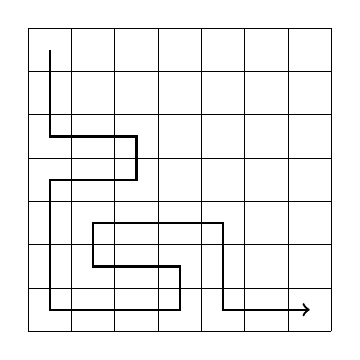
\begin{tikzpicture}[scale=.55]
  \begin{scope}
    \draw (0, 0) grid (7, 7);
    \draw[thick,->] (0.5,6.5) -- (0.5,4.5) -- (2.5,4.5) --
          (2.5,3.5) -- (0.5,3.5) -- (0.5,0.5) --
          (3.5,0.5) -- (3.5,1.5) -- (1.5,1.5) --
          (1.5,2.5) -- (4.5,2.5) -- (4.5,0.5) --
          (6.5,0.5);
  \end{scope}
\end{tikzpicture}
\end{center}
Sử dụng quan sát này, chúng ta có thể kết thúc tìm kiếm
ngay lập tức nếu chúng ta đến ô vuông dưới cùng bên phải quá sớm.
\begin{itemize}
\item
thời gian chạy: 119 giây
\item
số lượng lệnh gọi đệ quy: 20 tỷ
\end{itemize}

\subsubsection{Tối ưu hóa 3}

Nếu đường đi chạm vào một bức tường
và có thể rẽ trái hoặc phải,
lưới sẽ chia thành hai phần
chứa các ô vuông chưa được thăm.
Ví dụ, trong tình huống sau,
đường đi có thể rẽ trái hoặc phải:

\begin{center}
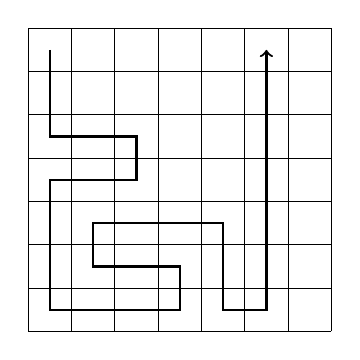
\begin{tikzpicture}[scale=.55]
  \begin{scope}
    \draw (0, 0) grid (7, 7);
    \draw[thick,->] (0.5,6.5) -- (0.5,4.5) -- (2.5,4.5) --
          (2.5,3.5) -- (0.5,3.5) -- (0.5,0.5) --
          (3.5,0.5) -- (3.5,1.5) -- (1.5,1.5) --
          (1.5,2.5) -- (4.5,2.5) -- (4.5,0.5) --
          (5.5,0.5) -- (5.5,6.5);
  \end{scope}
\end{tikzpicture}
\end{center}
Trong trường hợp này, chúng ta không thể thăm tất cả các ô vuông nữa,
vì vậy chúng ta có thể kết thúc tìm kiếm.
Tối ưu hóa này rất hữu ích:

\begin{itemize}
\item
thời gian chạy: 1.8 giây
\item
số lượng lệnh gọi đệ quy: 221 triệu
\end{itemize}

\subsubsection{Tối ưu hóa 4}

Ý tưởng của Tối ưu hóa 3
có thể được tổng quát hóa:
nếu đường đi không thể tiếp tục đi thẳng
nhưng có thể rẽ trái hoặc phải,
lưới sẽ chia thành hai phần
cả hai đều chứa các ô vuông chưa được thăm.
Ví dụ, hãy xem xét đường đi sau:

\begin{center}
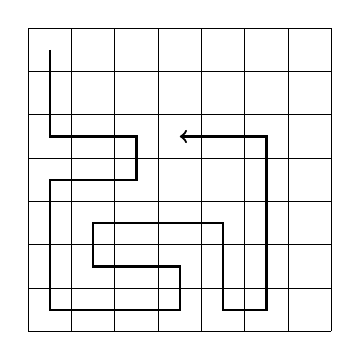
\begin{tikzpicture}[scale=.55]
  \begin{scope}
    \draw (0, 0) grid (7, 7);
    \draw[thick,->] (0.5,6.5) -- (0.5,4.5) -- (2.5,4.5) --
          (2.5,3.5) -- (0.5,3.5) -- (0.5,0.5) --
          (3.5,0.5) -- (3.5,1.5) -- (1.5,1.5) --
          (1.5,2.5) -- (4.5,2.5) -- (4.5,0.5) --
          (5.5,0.5) -- (5.5,4.5) -- (3.5,4.5);
  \end{scope}
\end{tikzpicture}
\end{center}
Rõ ràng là chúng ta không thể thăm tất cả các ô vuông nữa,
vì vậy chúng ta có thể kết thúc tìm kiếm.
Sau khi tối ưu hóa này, việc tìm kiếm trở nên
rất hiệu quả:

\begin{itemize}
\item
thời gian chạy: 0.6 giây
\item
số lượng lệnh gọi đệ quy: 69 triệu
\end{itemize}

~\\
Bây giờ là thời điểm tốt để ngừng tối ưu hóa
thuật toán và xem chúng ta đã đạt được gì.
Thời gian chạy của thuật toán ban đầu
là 483 giây,
và bây giờ sau các tối ưu hóa,
thời gian chạy chỉ còn 0.6 giây.
Do đó, thuật toán đã trở nên nhanh hơn gần 1000 lần
sau các tối ưu hóa.

Đây là một hiện tượng thông thường trong quay lui,
vì cây tìm kiếm thường lớn
và ngay cả những quan sát đơn giản cũng có thể hiệu quả
cắt tỉa tìm kiếm.
Đặc biệt hữu ích là các tối ưu hóa
xảy ra trong các bước đầu tiên của thuật toán,
tức là, ở đỉnh của cây tìm kiếm.

\section{Gặp nhau ở giữa}

\index{gặp nhau ở giữa}

\key{Gặp nhau ở giữa} là một kỹ thuật
trong đó không gian tìm kiếm được chia thành
hai phần có kích thước gần bằng nhau.
Một tìm kiếm riêng biệt được thực hiện
cho cả hai phần,
và cuối cùng kết quả của các tìm kiếm được kết hợp lại.

Kỹ thuật này có thể được sử dụng
nếu có một cách hiệu quả để kết hợp
kết quả của các tìm kiếm.
Trong tình huống như vậy, hai tìm kiếm có thể yêu cầu ít
thời gian hơn một tìm kiếm lớn.
Thông thường, chúng ta có thể biến một yếu tố $2^n$
thành một yếu tố $2^{n/2}$ bằng cách sử dụng kỹ thuật gặp nhau ở giữa.

Ví dụ, hãy xem xét một bài toán trong đó
chúng ta được cho một danh sách $n$ số và
một số $x$,
và chúng ta muốn tìm hiểu xem có thể
chọn một số số từ danh sách sao cho
tổng của chúng là $x$.
Ví dụ, cho danh sách $[2,4,5,9]$ và $x=15$,
chúng ta có thể chọn các số $[2,4,9]$ để có $2+4+9=15$.
Tuy nhiên, nếu $x=10$ cho cùng một danh sách,
không thể tạo thành tổng.

Một thuật toán đơn giản cho bài toán là
duyệt qua tất cả các tập con của các phần tử và
kiểm tra xem tổng của bất kỳ tập con nào có phải là $x$ không.
Thời gian chạy của một thuật toán như vậy là $O(2^n)$,
vì có $2^n$ tập con.
Tuy nhiên, bằng cách sử dụng kỹ thuật gặp nhau ở giữa,
chúng ta có thể đạt được một thuật toán hiệu quả hơn với thời gian $O(2^{n/2})$\footnote{Ý tưởng này
được giới thiệu vào năm 1974 bởi E. Horowitz và S. Sahni \cite{hor74}.}.
Lưu ý rằng $O(2^n)$ và $O(2^{n/2})$ là các
độ phức tạp khác nhau vì $2^{n/2}$ bằng $\sqrt{2^n}$.

Ý tưởng là chia danh sách thành
hai danh sách $A$ và $B$ sao cho cả hai
danh sách chứa khoảng một nửa số lượng số.
Tìm kiếm đầu tiên tạo ra tất cả các tập con
của $A$ và lưu trữ tổng của chúng vào một danh sách $S_A$.
Tương ứng, tìm kiếm thứ hai tạo ra
một danh sách $S_B$ từ $B$.
Sau đó, chỉ cần kiểm tra xem có thể
chọn một phần tử từ $S_A$ và một
phần tử khác từ $S_B$ sao cho tổng của chúng là $x$.
Điều này có thể xảy ra chính xác khi có một cách để
tạo thành tổng $x$ bằng cách sử dụng các số của danh sách ban đầu.

Ví dụ, giả sử danh sách là $[2,4,5,9]$ và $x=15$.
Đầu tiên, chúng ta chia danh sách thành $A=[2,4]$ và $B=[5,9]$.
Sau đó, chúng ta tạo các danh sách
$S_A=[0,2,4,6]$ và $S_B=[0,5,9,14]$.
Trong trường hợp này, tổng $x=15$ có thể được tạo thành,
vì $S_A$ chứa tổng $6$,
$S_B$ chứa tổng $9$, và $6+9=15$.
Điều này tương ứng với giải pháp $[2,4,9]$.

Chúng ta có thể cài đặt thuật toán sao cho
độ phức tạp thời gian của nó là $O(2^{n/2})$.
Đầu tiên, chúng ta tạo các danh sách \emph{đã sắp xếp} $S_A$ và $S_B$,
có thể được thực hiện trong thời gian $O(2^{n/2})$ bằng cách sử dụng một kỹ thuật giống như hợp nhất.
Sau đó, vì các danh sách đã được sắp xếp,
chúng ta có thể kiểm tra trong thời gian $O(2^{n/2})$ xem
tổng $x$ có thể được tạo từ $S_A$ và $S_B$ hay không.